\documentclass[a4]{article}
\usepackage[utf8]{inputenc}
\usepackage[T1]{fontenc}
\usepackage{fixltx2e}
\usepackage{graphicx}
\usepackage{longtable}
\usepackage{float}
\usepackage{wrapfig}
\usepackage[normalem]{ulem}
\usepackage{textcomp}
\usepackage{marvosym}
\usepackage{wasysym}
\usepackage{amssymb}
\usepackage{amstext}
\usepackage{hyperref}
\usepackage{color}
\usepackage{listings}

\newcommand{\todo}[1]{\textcolor{red}{\noindent$\rightarrow$ TODO: #1}}

\author{Zuhaitz Beloki and  Kike Fernández and Aitor Soroa\\\texttt{a.soroa@ehu.es}}
\date{\today}
\title{Newsreader virtual machine}

\definecolor{gray}{rgb}{0.4,0.4,0.4}
\definecolor{darkblue}{rgb}{0.0,0.0,0.6}
\definecolor{cyan}{rgb}{0.0,0.6,0.6}
\definecolor{maroon}{rgb}{0.5,0,0}
\definecolor{darkgreen}{rgb}{0,0.5,0}

\lstdefinelanguage{XML}
{
  basicstyle=\ttfamily\small,
  morestring=[s]{"}{"},
  morecomment=[s]{?}{?},
  morecomment=[s]{!--}{--},
  commentstyle=\color{darkgreen},
  moredelim=[s][\color{black}]{>}{<},
  moredelim=[s][\color{darkgreen}]{\ }{=},
  stringstyle=\color{blue},
  identifierstyle=\color{maroon}
}

\lstset{language=XML}

\begin{document}

\maketitle
\tableofcontents
\cleardoublepage


\section{NewsReader architecture for distributed NLP processing}
\label{sec:newsr-arch-distr}

\begin{figure}[t]
  \centering
  {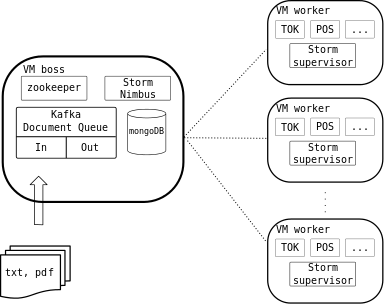
\includegraphics[scale=0.5]{lpstageVM14a.png}}  
  \caption{Main architecture of the NWR distributed pipeline}
  \label{fig:main-arch-nwr}
\end{figure}

This document describes the distributed pipeline implemented within the
NewsReader project. The pipeline follows an streaming computing
architecture, where the computation is not limited to any
timeframe. Instead, the pipeline is always waiting to the arrival of new
documents, and one such new document arrives the NLP processing starts.

Figure \ref{fig:main-arch-nwr} shows a general overview of the NewsReader
distributed pipeline. The processing NLP modules and the software
infrastructure for performing parallel and distributed streaming processing
of documents is packed into virtual machines (VM). Specifically, we
distinguish two types of VM into the cluster:
\begin{itemize}
\item One ``boss'' node, which is the main entry of the documents and which
  supervises the processing.
\item Several ``worker'' nodes, which actually perform the NLP processing.
\end{itemize}

The boss node is the entry point for input documents. It contains a document
queue where the input documents are stored and wait until they enter the
pipeline. It also supervises the execution of the different stages of the
processing pipeline. When the NLP processing is over, the boss node receives
the processed NAF document into the output queue, and writes it in a
specified directory.

The boss node implements a REST service that accept documents to the
processing pipeline. For instance, the following command sends the document
\texttt{doc.xml} to the processing pipeline\footnote{In this document we
  will show many examples which are commands to execute from the CLI. If the
  command has to be executed from the host machine, we will use the '\%'
  character in the beginning of the line. If the command is meant to be
  executed from the boss machine, we will use the '\$' character.}:

\begin{verbatim}
% curl --form "file=@doc.xml" http://BOSSIP:80/upload_file_to_queue.php
\end{verbatim}

Once the NLP processing is finished, the final NAF will be stored inside the
boss VM, under the \texttt{docs/output} directory. In principle those
documents should be sent to the KnowledgeStore (KS), but at the time being
this last module which populates the KS with the processed NAFs is not
ready.

The worker nodes are the nodes where the NLP modules are executed. There can
be many worker nodes in a cluster, and therefore there can be many instances
of the modules running in parallel.

This document is a reference guide that covers the most important steps to
build a NewsReader architecture from scratch.

\section{VM from scratch}
\label{sec:vm-from-scratch}

We distribute a set of scripts with the aim of automatically create a fully
working cluster for distributed NLP processing. We call these scripts ``VM
from scratch'', as they create and configure the required virtual
machines. The scripts are in a github repository, at this address:

\begin{center}
  \texttt{https://github.com/ixa-ehu/vmc-from-scratch}
\end{center}

The latest version of the documentation is also in the same repository,
under the \texttt{doc} directory.

Creating a cluster using the scripts involves three main steps:
\begin{enumerate}
\item Create a basic cluster with the boss node and one worker node.
\item Make as many copies as required of the worker node.
\item Deploy the worker copies among different hosts and run the cluster.
\end{enumerate}

The subsections below will describe how to use the provided scripts to
achieve these goals in turn.

\subsection{Create a basic cluster}
\label{sec:create-basic-cluster}

The first step is to create the basic cluster using the
\texttt{create\_basic\_cluster.pl} script. Please note that the VM images
created by these scripts are huge (9 Gb memory), as they contain all the NLP
modules of the Newsreader processing pipeline. Likewise, the machine to
install those VMs need to have a large amount of RAM memory, as each VM,
particularly the worker nodes, need circa 14Gb of memory to run.

The script is executed as follows\footnote{In ubuntu machines, install the
  following packages before running this script
  \begin{itemize}
  \item libvirt-bin
  \item libguestfs-tools
  \item qemu-kvm
  \end{itemize}
\noindent besides, you'll need to run\\
\texttt{\% sudo update-guestfs-appliance}
}:

\begin{verbatim}
% sudo ./create_basic_cluster.pl --boss-ip 192.168.122.111 --boss-name bossvm \\
  --worker-ip 192.168.122.112 --worker-name workervm1
\end{verbatim}

\noindent The script needs four parameters:
\begin{itemize}
\item \texttt{--boss-ip} (\textbf{required}) the IP address of the boss
  VM\footnote{In this example and in the examples below we will use private
    IP addresses for the boss and worker IPs. See section
    \ref{sec:deploting-worker-vms} for more information about IP
    addresses.}.
\item \texttt{--boss-name} (\textbf{required}) the hostname of the boss VM
\item \texttt{--worker-ip} (\textbf{required}) the IP address of the first
  worker VM created by this script.
\item \texttt{--worker-name} (\textbf{required}) the hostname of the worker
  VM.
\item \texttt{--master-ip} (\textbf{optional}) the IP address of the IXA
  master machine. This machine is where the latest version of all NLP
  modules are.
\end{itemize}

Use the \texttt{--help} option to obtain information about the script's
parameters (this option is present in all scripts described here).

The script will perform the following steps for creating the basic cluster:
\begin{itemize}
\item Copy an empty VM image from the IXA servers.
\item Create the boss VM image using the empty VM image. In the example
  above, the hostname of the boss VM is ``\textrm{bossvm}'' and its IP
  address is \texttt{192.168.122.111}.
\item Create the worker VM image using the empty VM image.  In the example
  above, the hostname of this worker VM is ``\textrm{workervm1}'' and its IP
  address is \texttt{192.168.122.112}.
\item The VMs have an unique user ``\texttt{newsreader}'' whose password is
  ``\texttt{readNEWS89}''. The user can \texttt{sudo} any root commands
  inside the VMs.
\end{itemize}

The next step is to turn on both VMs and start a synchronization process so
that the required software (both the system software as well as the NLP
modules) is properly installed in the newly created VMs.

The above script creates two XML definition files with the specification of
the boss and worker virtual machines\footnote{See section \ref{sec:virtual-machines-xml} on the XML
  definitions of the VMs.}. To (locally) run the VMs, run the following
commands as root from the host machine:

\begin{verbatim}
% virsh create nodes/bossvm.xml
% virsh create nodes/workervm1.xml
\end{verbatim}

Once the machines are up and running, we ssh into the boss VM.

\begin{verbatim}
% ssh newsreader@192.168.122.111
(pass: readNEWS89)
\end{verbatim}

Once logged into the boss VM, run the following:

\begin{verbatim}
$ sudo /root/init_system.sh -l {en|es}
\end{verbatim}
%$

Select \texttt{-l en} to download and install the english NLP modules, and \texttt{-l es} for spanish modules.

This command prepares installs all required software into both virtual
machines (boss and worker). Specifically, the script performs the following steps:
\begin{itemize}
\item Install the required software into the boss VM. This involves the
  installation, among others, of the following packages:
  \begin{itemize}
  \item \emph{Zookeeper}
  \item \emph{Storm}
  \item \emph{Kafka}
  \item \emph{MongoDB}
  \item \emph{Puppet}
  \end{itemize}
\item Synchronize the boss VM with the IXA master VM to obtain all the NLP
  modules.
\item Synchronize the worker VM with the boss VM to obtain a copy of all the
  NLP modules.
\item Start the \emph{puppet} agents on both the boss and worker VMs.
\end{itemize}

When the scripts finalizes the basic cluster is finally created and
configured. The boss VM image is stored in the file
\texttt{nodes/bossvm.img} and the worker image is
\texttt{nodes/workervm1.img}. The cluster is already ready for processing
documents, although it does not make much sense to use a cluster with a
single worker node. Therefore, the next step is to create the required
copies of the worker VMs.

\subsection{Making copies of worker VMs}
\label{sec:making-copies-worker}

The next step is thus to copy the worker VM and create new worker nodes in
the cluster. Before doing this, however, the boss and the worker VMs must be
shut down. There are several ways to shut down the cluster. One possible way
is, being into the boss VM, is to execute the following:

\begin{verbatim}
$ sudo pdsh -w workervm1 poweroff
$ sudo poweroff
\end{verbatim}

The first command remotely shuts down the worker VM, whereas the second
command shuts down the boss VM itself. In any case, check that the VMs are
properly shut down by executing the \texttt{sudo virsh list} command from
the host machine. The command should return an empty list of VMs:

\begin{verbatim}
% sudo virsh list
 Id    Name                           State
----------------------------------------------------
\end{verbatim}


Once the cluster shut down, one can make as many copies as wanted of the
worker nodes. The script \texttt{cp\_worker.pl} accomplishes this task:

\begin{verbatim}
%  sudo ./cp_worker.pl --boss-img nodes/bossvm.img \
  --worker-img nodes/workervm1.img 192.168.122.113,workervm2
\end{verbatim}

The script needs two parameters with the images of the boss VM and the first
created worker VM (\texttt{workervm1} in our example). Then, the script
accepts a space separated list of \texttt{IP,hostname} pairs. The above
example just creates a copy of the worker VM, called \texttt{workervm2},
whose IP address will be \texttt{192.168.122.102}. Of course, it is very
important that each VM receives a different hostname and IP address. 

If we were to create more copies of the VM, we can just run the script
again, the only requisite being that the cluster VM can not be running. For
instance, the following command will create two more worker nodes:

\begin{verbatim}
%  sudo ./cp_worker.pl  --boss-img nodes/bossvm.img \
  --worker-img nodes/workervm1.img \
  192.168.122.114,workervm3 192.168.122.115,workervm4
\end{verbatim}

After this step we need to boot the cluster manually. Section
\ref{sec:boot-stopp-clust} explains how to power on and power off the whole
cluster at any time.

\subsubsection*{Creating copies of the worker without stopping the cluster}
\label{sec:creat-copi-work}

The requirement of having to stop the cluster before making copies of the
workers may too hard to fulfill, in the case the cluster is running and
processing documents. Therefore, we present a method to create worker
nodes without the need to stop the whole cluster. However, this method needs
a copy of a worker image, and it is very important that this particular
image is not running.

For creating a worker without stopping the cluster, execute the following:

\begin{verbatim}
%  sudo ./cp_worker.pl  --boss-img nodes/bossvm.img \
  --worker-img nodes/workervm1.img \
  192.168.122.116,workervm5
\end{verbatim}

This will create the new \texttt{workervm5} node with IP address
\texttt{192.168.122.116}. Now, we need to log into the boss node, and
manually add this new address to the \texttt{/etc/hosts} file:

\begin{verbatim}
% sudo echo "192.168.122.116	workervm5" >> /etc/hosts
\end{verbatim}

The next step is to stop the topology (see section
\ref{sec:running-topology}) and run it again with the proper number of
workers/CPUs.

\subsection{Virtual machines XML definitions}
\label{sec:virtual-machines-xml}

The virtual machines specifications are defined in a XML document, one
document per VM. These XML specification document is stored along with the
VM image, i.e., if the image is in \texttt{nodes/workervm1.img}, the
corresponding XML specification is \texttt{nodes/workervm1.xml}. You may
want to manually edit the XML specification file to change some important
things:
\begin{itemize}
\item The number of CPUs assigned to the VM (line 6, \texttt{/domain/vcpu}
  element). By default VMs are assigned 1 CPU but this can be easily
  changed. In fact, \textbf{we recommend to increase the number of CPUs per
    worker whenever possible}.
\item The memory assigned to the VM (line 4, \texttt{/domain/memory}
  element). By default VMs are assigned 14Gb of RAM (needed mostly by
  the NED module). The boss VM does not need more than 3Gb of memory,
  but this must be fixed manually. If you plan to set more than one
  worker VM, we recommend creating a dedicated VM for the NED module,
  as explained in section \ref{sec:dedicated}.
\item The exact location of the image files (line 22,
  \texttt{/domain/devices/disk/source} element). If you plan to deploy the
  worker VM on a different machine, you must change this value to
  the directory where the worker image file will be.
\end{itemize}

% You can even create a template XML document with the appropriate CPU/memory
% values and use this template when creating the VMs. First, copy the template
% file provided with the scripts:

% \begin{verbatim}
% % cp templates/vmdef/def.xml templates/vmdef/myworkers.xml
% \end{verbatim}

% Now you can edit the template and change the CPU and VM names

% runCommand("sed -i 's/_VM_NAME_/".$boss_name."/g' ".$Bin."/nodes/".$boss_name.".xml");
% runCommand("sed -i 's/_UUID_/".$uuid."/g' ".$Bin."/nodes/".$boss_name.".xml");
% runCommand("sed -i 's/_IMG_PATH_/".$Bin_f."\\/nodes\\/".$boss_name.".img/g' ".$Bin."/nodes/".$boss_name.".xml");
% runCommand("sed -i 's/_MACADDR_/".$boss_mac."/g' ".$Bin."/nodes/".$boss_name.".xml");

\subsection{Booting and stopping the cluster}
\label{sec:boot-stopp-clust}

Boot the boss VM by running this into the host machine:
	
\begin{verbatim}
% sudo virsh create nodes/bossvm.xml
\end{verbatim}
	
The host needs some time to start all the required services. To be
completely sure that the machine is ready, run the following command inside
the boss machine until it produces some output. First ssh into the boss VM,
and then:

\begin{verbatim}
$ ps -aux | grep zoo | grep java
\end{verbatim}
%$

Once the boss is ready, turn on the worker nodes running the following
inside the host machine:

\begin{verbatim}
% sudo virsh create nodes/workervm1.xml
% sudo virsh create nodes/workervm2.xml
...
\end{verbatim}

The above commands will start the worker VMs in turn. Each VM needs some
time to boot up (mostly due to the required time in loading the NED
module). Section \ref{sec:know-which-mach} explains how to know which
machines are connected to the boss VM.

\subsection{Deploying worker VMs into different host machines}
\label{sec:deploting-worker-vms}

In principle the worker VMs can be executed in any host machine, as far as
the host has a 64 bit CPU. The main requirement is that the IP of the worker
VM, as specified when creating the VM image, is accessible from within the
boss VM. Likewise, the boss IP has to be accessible from the worker VM.

In the examples on this document all the IPs are private IPs, and therefore
not accessible from outside the host machine. If you need to copy the worker
VMs among several host machines, perhaps the best way is to use a bridged
network configuration (not explained here). Alternatively, you can use
iptables for allowing external access through ssh to the VM. In any case,
talk with the IT people in your laboratory to correctly set-up the
environment.

\subsection{Knowing which machines are connected to the boss VM}
\label{sec:know-which-mach}

When the cluster is up and running, we can consult any time which worker
machines are connected to the boss. This is easily done by querying the
STORM server on the boss VM. From inside the boss VM, run the command line
``elinks'' web browser:

\begin{verbatim}
$ elinks localhost:8080
\end{verbatim}
%$

Another option is to connect to the boss VM from the host machine, by
putting the address \texttt{http://ip\_of\_boss:8080}. In the running example
used in this document the boss IP is 192.168.122.111, we should put the
address \texttt{http://192.168.122.111:8080} into the web browser.

\section{Running the topology}
\label{sec:running-topology}

The steps described in section \ref{sec:vm-from-scratch} will create a
cluster that is ready to start the NLP processing. For this, we need first
to load a topology into the cluster. The topology is an abstraction that
describes processing steps each document passes through. In principle the
cluster can run any topology, the only requisite being that the NLP modules
described in the topology are installed in the worker VMs.

Topologies are declaratively described in an XML document. There are already
some topologies in the bossvm \texttt{opt/topologies/specs} directory. In
this example, we will run the topology described in
\texttt{opt/topologies/specs/test.xml}. 

Apart from the topology definition, running the topology requires knowing
the number of worker nodes in the topology, and the number of CPUs used. In
the running example of this document we are using three workers. Suppose we
also use two CPUs per worker\footnote{Section \ref{sec:virtual-machines-xml}
  describes how to change the number of CPUs assigned to a node}. So, the
total of CPUs assigned to worker nodes is $6$. This parameter is very
important because it fixes the maximum parallelization we can achieve. If we
have 6 CPUs working on our cluster, it makes little sense to have more than
6 copies of any NLP module running in parallel.

Inside the boss VM, run the following to run the topology:

\begin{verbatim}
$ opt/sbin/run_topology.sh -g 6 -s opt/topologies/specs/test.xml
\end{verbatim}
%$

This will load the topology and, as a consequence, the cluster will be ready
to accept and process documents.

The script also accepts another optional parameter to specify the main
configuration of the topology, the default value being
\texttt{opt/etc/topology/topology.conf}. This configuration file is
seldom changed within the newsreader project, and specifies values
such as the port and addresses of various services such as zookeeper,
rabbitmq, mongoDB, etc. However, there is one parameter that need to
be checked. The ``host'' values (\texttt{zookeeper.host},
\texttt{mongodb.host}) need to point to the hostname of the boss node
(by default, \texttt{bossvm}).

\subsection{Topology XML specification}
\label{sec:topol-xml-spec}

The topology executed by the cluster is declaratively defined in an XML
document. Here is an excerpt of a small topology:

\begin{lstlisting}
<topology>
  <cluster componentsBaseDir="/home/newsreader/components"/>
  <module name="EHU-tok" runPath="EHU-tok/run.sh"
          input="raw" output="text"
          procTime="10"/>
  <module name="EHU-pos" runPath="EHU-pos/run.sh"
          input="text" output="terms"
          procTime="15" source="EHU-tok"/>
  <module name="EHU-nerc" runPath="EHU-nerc/run.sh"
          input="terms" output="entities"
          procTime="75" source="EHU-pos"/>
</topology>
\end{lstlisting}

The \texttt{<cluster>} element specifies the base directory of the NLP
modules. Each module is described by a \texttt{<module>} element, whose
attributes are the following:

\begin{itemize}
\item \texttt{name} (\textbf{required}): the name of the module.
\item \texttt{runPath} (\textbf{required}): the path relative to \texttt{componentsBaseDir}
  where the module resides.
\item \texttt{input} (\textbf{required}): a comma separated list of NAF layers required by the
  module as input.
\item \texttt{output} (\textbf{required}): a comma separated list of NAF layers produced by the
  module.
\item \texttt{source} (optional): the previous module in the pipeline. If
  absent, the attribute will get the value of the immediately preceding it
  according to the XML tree. If the module is the first node in the XML
  tree, and the source attribute is absent, the attribute gets no value at
  all.
\item \texttt{procTime} (optional): the percentage of time this particular
  module uses when processing a document.
\item \texttt{numExec} (optional): the number of instances of the module
  that will run in parallel.
\item \texttt{vm\_type} (optional): the type of dedicated machines this
  module will be run on (see section \ref{sec:dedicated}).
\end{itemize}

The topology is defined by looking at the chains of \texttt{source}
attributes among the modules, which have to define a directed acyclic
graph. The module without parents is considered to be the first module in
the pipeline. Likewise, the module without children is the last module in
the pipeline. In principle the declaration may define non linear topologies,
but at the moment its use is not properly tested, and thus not recommended.

The last two attributes are very important and require some tuning in order
to obtain the maximum efficiency when processing the documents. There are
two ways of calculating these factors. If the \texttt{numExec} parameter is
present, this particular number of instances will be used. If
\texttt{numExec} is absent, the system will use the \texttt{procTime}
information, along with the number of nodes/CPUs to automatically calculate
the number of instances of each module. The main idea is to execute as many
copies as possible of the most resource demanding modules. Finally, if both
\texttt{numExec} and \texttt{procTime} are absent, the system will run one
single instance of the module.


\subsection{Dedicated VMs}
\label{sec:dedicated}

Dedicated VMs are those which only run certain modules of the
pipeline. For instance, we recommend to have a dedicated VM which only
runs the NED module, and assign 10GB to it. Then, the rest of VMs
would not need to run the NED module and would not need more than
5GB\footnote{Run 'sudo supervisorctl stop spotlight' command to stop
  the NED process}.

Follow the steps below to create a dedicated VM:

\begin{enumerate}
\item Edit the Storm config file of the VM
  (/opt/storm/config/storm.yaml), and add the following lines:

  \begin{verbatim}
    supervisor.scheduler.meta:
      vm_type: "WORKER_TYPE"  # Create your own worker types here
  \end{verbatim}

\item Restart storm-supervisor process running the following command:

\begin{verbatim}
  $ sudo supervisorctl restart storm-supervisor
\end{verbatim}

\item In topology spec file
  (~/opt/topologies/specs/nwr\_v30\_nonlinear.xml), set the 'vm\_type'
  attribute to each module to be run on the dedicated machine. For
  instance, in the following topology we are defining that the EHU-ned
  module will run on any dedicated VM of type "NEDWorker":

  \begin{lstlisting}
<topology>
  <cluster componentsBaseDir="/home/newsreader/components"/>
  <module name="EHU-tok" runPath="EHU-tok/run.sh"
          input="raw" output="text"
          procTime="10"/>
  <module name="EHU-pos" runPath="EHU-pos/run.sh"
          input="text" output="terms"
          procTime="15" source="EHU-tok"/>
  <module name="EHU-nerc" runPath="EHU-nerc/run.sh"
          input="terms" output="entities"
          procTime="75" source="EHU-pos"/>
  <module name="EHU-ned" runPath="EHU-ned/run.sh"
          input="entities" output="entities"
          procTime="15" source="EHU-nerc" vm_type="NEDWorker"/>
</topology>
\end{lstlisting}

\item Run the topology choosing the number of general use (-g) and
  dedicated (-d) CPUs. For instance:

\begin{verbatim}
   $ opt/sbin/run_topology.sh -g 6 -d 1 -s opt/topologies/specs/nwr_v30_nonlinear.xml
\end{verbatim}

  \texttt{Note: Any topology running should be killed before running a
    new topology. Use the kill\_topology.sh script located in opt/sbin
    to kill them.}
\end{enumerate}


\section{Troubleshooting and tools}
\label{sec:troubl-tools}

This section describes the most usual tasks performed by the cluster
administrator to manage and monitorize the cluster, as well as when facing
many problems that may occur. In principle the cluster should run flawlessly
and without errors; it should just accept documents via the boss input port
or inside the boss machine itself, and the documents should get processed,
put in the output queue of the boss machine, and written to the
\texttt{docs/output} in the boss machine. However, if something goes wrong
there are some useful commands to help understanding what is happening.



\subsection{Synchronizing the modules}
\label{sec:synchr-modul}

The NLP modules are constantly being developed and upgraded into the IXA
master machine. Obtaining the latest version of the modules from the master
node into the cluster involves two steps. First, synchronize the boss node
with the IXA master node; then, synchronize each worker node with the boss
node.

For synchronizing the boss node with the IXA master, log in into the boss VM
and run the following:

\begin{verbatim}
$ sudo ./update_nlp_components_boss.sh -l {en|es}
\end{verbatim}
%$

The language is selected with the argument \texttt{-l}. The value \texttt{en} means the english modules will be downloaded. In the case of the value \texttt{es}, spanish modules will be downloaded.

For updating the workers there are two main options. One option is to log in
into each of the workers and execute the following:

\begin{verbatim}
$ sudo ./update_nlp_components_worker.sh
\end{verbatim}
%$

The other is to update the worker nodes from inside the boss node, using the
\texttt{pdsh} command. Being logged into the boss machine, run the
following for each worker node:

\begin{verbatim}
$ sudo pdsh -w ip_of_worker /home/newsreader/update_nlp_components_worker.sh
\end{verbatim}
%$

\subsection{Document queue}
\label{sec:document-queue}

The boss VM contains two document queues, for input and output NAF
documents, respectively. The input queue stores the documents to be
processed until they are consumed by the NLP pipeline. The output queue
stores the final NAF documents.

In principle, the usage of the queues is wholly automatic. The user sends a
document to the input queue, and eventually the processed document is
enqueued into the output queue. However, it is important to have some basic
notions about how these queues are implemented in case we want to consult
the contents of a particular queue, or if we want to manually send or
retrieve documents.

The queues are implemented using
``RabbitMQ''\footnote{\url{https://www.rabbitmq.com/}}. RabbitMQ is a
messaging system that can be distributed among many machines and that
provides fast and reliable access to the queue contents. In NewsReader
we have two queues, called ``\texttt{input\_queue}'' and
``\texttt{output\_queue}'', respectively. Once a document is sent to
the queue, it stays there for a specific time frame, which by default
is set to seven days. The input queue is attached to a consumer that
continually pulls documents from the queue and sends them to the first
stage of the processing pipeline.

Inside the boss VM there are some tools which can help with the management
of the queues. Currently there exist the following tools:

\subsection*{\texttt{push\_queue}}
\label{sec:send-to-queue.pl}

This tool is useful for feeding the input queue with documents from inside
the \textrm{boss} VM. The usage is as follows:

\begin{verbatim}
$ opt/sbin/push_queue -f docs/input/input.xml
\end{verbatim}
%$

Please note that documents can be sent to the input queue from outside the
\textrm{boss} VM, by using the following command:

\begin{verbatim}
% curl --form "file=@input.xml" http://BOSSIP:80/upload_file_to_queue.php
\end{verbatim}

% \todo{check port, service}

\noindent this is meant to be the principal way to send documents into the
NewsReader pipeline. The \texttt{push\_queue} tool is an auxiliary tool
for manually feeding the input queue with new documents.

% LS_QUEUE: RabbitMQn inplementatu gabe!
%
% \subsection*{\texttt{ls\_queue}}
% \label{sec:ls_queue}

% Sometimes it is useful to know which documents are present in a queue (input
% or output), and the \texttt{ls\_queue} command does exactly this. This is a
% typical example of usage (from inside the \textrm{boss} VM):

% \begin{verbatim}
% $ opt/sbin/ls_queue
% doc18.txt  1209  9   input_queue
% doc20.txt  1025  10  input_queue
% doc23.txt  2020  11  input_queue
% doc24.txt  347   12  input_queue
% doc26.txt  789   13  input_queue
% doc27.txt  257   14  input_queue
% doc28.txt  1675  15  input_queue
% doc29.txt  9837  16  input_queue
% doc20.txt  721   17  input_queue
% \end{verbatim}
% %$

% The tool displays 4 columns for each document in the queue, namely, the
% document name, the size, the offset number, and the queue name.

% The above example showed the documents of the input queue waiting to be
% processed. The ``\texttt{-a}'' switch shows all the documents in the
% queue. Remember that Kafka keeps all documents in the queues for some time
% (by default, seven days). The following command shows all the documents in
% the queue.

% \begin{verbatim}
% $ opt/sbin/ls_queue -a
% doc1.txt   762   1   input_queue
% doc0.txt   4678  2   input_queue
% doc3.txt   9876  3   input_queue
% doc4.txt   189   4   input_queue
% doc6.txt   875   5   input_queue
% doc7.txt   8989  6   input_queue
% doc8.txt   6735  7   input_queue
% doc9.txt   9875  8   input_queue
% doc18.txt  1209  9   input_queue
% doc20.txt  1025  10  input_queue
% doc23.txt  2020  11  input_queue
% doc24.txt  347   12  input_queue
% doc26.txt  789   13  input_queue
% doc27.txt  257   14  input_queue
% doc28.txt  1675  15  input_queue
% doc29.txt  9837  16  input_queue
% doc20.txt  721   17  input_queue
% \end{verbatim}
% %$

% It is also possible to list the documents of the output query, using the
% ``\texttt{-q}'' command switch to select the queue name:

% \begin{verbatim}
% $ opt/sbin/ls_queue -q output_queue
% doc1.txt_065a4fe5686a240b0569d35c6f04b025.naf 222715  21   output_queue
% doc0.txt_0ff7e7f4e55ad14f085aada286f0b718.naf 219339  22   output_queue
% doc3.txt_2ab255aac76c7b7110be1fe7cf9bfd0e.naf 214548  23   output_queue
% doc4.txt_3762e590fe5ba62e96845491acda0656.naf 213492  24   output_queue
% doc6.txt_98aef58c8b9b824006dd3c5a0d4d87cb.naf 212985  25   output_queue
% doc7.txt_d0af8c39cd227492e6d6cf656be19491.naf 211940  26   output_queue
% doc8.txt_45d6c827fbab1ef8f211a2a0ed2d448c.naf 210390  27   output_queue
% doc9.txt_5cd1fbedf874d25391ba78ea789ebe90.naf 209767  28   output_queue
% doc18.tx_621f460498502b42d4a9ddf2401349f9.naf 209104  29   output_queue
% \end{verbatim}
% %$

% Note that these examples show documents consumed from the input queue are
% already processed and stored in the output queue.

\subsection*{\texttt{flush\_queue}}
\label{sec:flush_queue}

Once the documents are processed, they are stored in the output queue. The
boss machine contains a consumer that continuously pulls from the output
queue and stores the documents in the \texttt{docs/output}
directory. However, sometimes it is interesting to dump all the current
content of a queue (input or output) into a directory. The
\texttt{flush\_queue} accomplishes this task.

\begin{verbatim}
$ opt/sbin/flush_queue -q output_queue -o path_to_docs
\end{verbatim}
%$

The parameters of the script are the following:
\begin{itemize}
\item \texttt{-o} (\textbf{required}): the directory to dump the documents.
\item \texttt{-q} (optional): the queue to flush. If omitted, the script
  dumps the document from the \texttt{output\_queue} queue.
\end{itemize}

\subsection*{Logs}
\label{sec:logs}

The cluster maintains a log of all the documents when passing over the
several stages of the pipeline. Each time the document processing starts, or
when it enters some particular stage of the topology (in any worker
machine), a log entry is created. Besides, if a document processing fails a
record is created with the name of the document and the module which caused
the error.

All the log records are stored into the \emph{mongoDB} database, and are
accessible from within the boss node. To access the logs, one has to first
enter the so called mongo shell. Being logged into the boss machine, run the
\texttt{mongo} command:

\begin{verbatim}
$ mongo
MongoDB shell version: 2.4.6
connecting to: test
> use newsreader-pipeline
switched to db newsreader-pipeline
> db.log.find()
\end{verbatim}
%$

the \texttt{find} command will show all entries of the log database. Each
log entry has the following fields:
\begin{itemize}
\item \texttt{\_id}: internal ID.
\item \texttt{tag}: the entry type. Possible values:
  \begin{itemize}
  \item \texttt{DOC\_START}    -> the document "doc\_id" enters the pipeline
  \item \texttt{DOC\_BOLT\_RCV} -> the document "doc\_id" enters the bolt  "module\_id"
  \item \texttt{DOC\_BOLT\_EMT} -> the document "doc\_id" exits the "module\_id"
  \item \texttt{DOC\_BOLT\_FAIL} -> the document name "doc\_id" failed in bolt "module\_id"
  \item \texttt{DOC\_FAIL} -> the document "doc\_id" failed
  \item \texttt{DOC\_ACK} -> the document "doc\_id" worked as expected
  \end{itemize}
\item \texttt{doc\_id}: the document name.
\item \texttt{module\_id}: the NLP module.
\item \texttt{hostname}: the node name.
\item \texttt{timestamp}: the time stamp in mongoDB format.
\end{itemize}

\subsubsection*{Find documents with errors, also displaying the bolt which caused the error and the worker node}

\begin{verbatim}
> db.log.find( { tag: "DOC_BOLT_FAIL" }, { _id:0, doc_id:1, module_id:1, hostname:1 } )
{ "doc_id" : "4MSN-CTV0-TX2J-N1W8_8bb9805598b55e10850852165981897f.xml", 
  "module_id" : "FBK-time", "hostname" : "workervm1" }
{ "doc_id" : "4MR6-N790-TX33-71WM_bab251443f3e6869306c87f8173e11c4.xml", 
   "module_id" : "EHU-corefgraph", "hostname" : "workervm2" }
{ "doc_id" : "4MRN-CMP0-TX37-G2P3_82436b4a93ef1826a280763ac2838a74.xml", 
   "module_id" : "EHU-corefgraph", "hostname" : "workervm1" }
{ "doc_id" : "4MRP-5X50-TX2J-N2H8_d83f60a3c7a5e783b8e84fd5d13a9b69.xml", 
   "module_id" : "EHU-corefgraph", "hostname" : "workervm3" }
...
\end{verbatim}

\subsubsection*{Find successfully analyzed documents}

\begin{verbatim}
> db.log.find( { tag: "DOC_ACK" }, { _id:0, doc_id:1 } )
{ "doc_id" : "4MR1-81M0-TWX2-W2WD_f5341438336a8f739fd3bb2192a3374b.xml" }
{ "doc_id" : "4MR2-D9G0-TX52-F26P_5484c46f08a6242518fa389f8f1e4851.xml" }
{ "doc_id" : "4MRC-JSD0-TX2J-N1V0_7a5dc0f87c195104251969c9ca100c6c.xml" }
{ "doc_id" : "4MRK-J360-TX2J-N39T_f51f321d7a7a60d8c802bfece498027b.xml" }
...
\end{verbatim}

\subsection{Starting and stopping the services}
\label{sec:start-stopp-serv}

There are a number of scripts in the boss VM (under the \texttt{opt/init.d}
directory) to start and stop many services. It is convenient to stop the
puppet agent before stopping services:

\begin{verbatim}
$ sudo /etc/init.d/puppet stop
\end{verbatim}
%$

Likewise, the puppet agent needs to be restarted after the services are
running again:

\begin{verbatim}
$ sudo /etc/init.d/puppet start
\end{verbatim}
%$

Here is a list of the provided scripts to start or stop the services. All
these scripts require one command, \texttt{start} or \texttt{stop}, which
starts or stops the service, respectively:
\begin{itemize}
% \item \texttt{kafka\_server}: it needs a parameter, \texttt{start} or
%   \texttt{stop}. The script starts or stops the kafka service (document
%   queues), respectively.
\item \texttt{zookeeper\_server}: start or stop the zookeeper service.
\item \texttt{storm\_boss\_server}: start or stop the STORM nimbus service.
\item \texttt{boss\_servers}: this script start or stops all services in the
  boss VM.
\item \texttt{wipe\_all\_boss}: this script is special and erases all
  documents of the queues. \textbf{Use it with care}! It is recommended to
  first dump the documents of the queues in some temporary directory before
  erasing the queues.
\end{itemize}

The worker services can also be started/stopped:
\begin{itemize}
\item \texttt{worker\_servers}: start or stop all the services in the worker
  VM. Run this script inside the worker VM. Alternatively, run this script
  from inside the boss VM using the \texttt{pdsh} tool. Inside the boss VM,
  write the following:
\begin{verbatim}
$ sudo pdsh -w ip_of_worker /home/newsreader/opt/sbin/worker_servers stop
$ sudo pdsh -w ip_of_worker /home/newsreader/opt/sbin/worker_servers start
\end{verbatim}
%$
\end{itemize}


\end{document}

%%% Local Variables:
%%% mode: latex
%%% TeX-master: t
%%% End:
